\documentclass[12pt,oneside, a4paper]{book}
\usepackage[utf8]{inputenc}
\usepackage[croatian]{babel}
\usepackage[margin=1in]{geometry}
\usepackage{multirow}
\usepackage{textcomp}
\usepackage{gensymb}
\usepackage{bigstrut}
\usepackage{amsmath}
\usepackage{amsfonts}
\usepackage{amssymb}
\usepackage[hidelinks]{hyperref}
\usepackage{enumitem}
\usepackage{lmodern}
\usepackage{datetime}
\usepackage{pgfplots}
\usepackage{tikz}
\usepackage{listings}
\usepackage{color}
\usepackage{float}
\usepackage{fancyhdr} 
\usepackage{titlesec}
\usepackage{pdflscape}
\pgfplotsset{compat=1.16}
\usepackage{nomencl}
\usetikzlibrary{automata, positioning, arrows.meta}
\usepackage{caption}
\captionsetup{justification=centering}

\pagestyle{plain}

\renewcommand{\headrulewidth}{0pt}
\renewcommand{\footrulewidth}{0pt}

\fancypagestyle{plain}
\fancyhf{}

\usepackage{array}

\newcolumntype{L}[1]{>{\raggedright\arraybackslash}p{#1}}
\newcolumntype{C}[1]{>{\centering\arraybackslash}p{#1}}

\lstset{
  basicstyle=\ttfamily\small,
  frame=single,
  breaklines=true,
  showstringspaces=false,
  aboveskip=1em,
  belowskip=1em,
  captionpos=b,
}
\lstdefinestyle{shell}{
  basicstyle=\ttfamily\small,
  frame=single,
  backgroundcolor=\color{gray!5},
  breaklines=true,
  showstringspaces=false
}
\captionsetup[lstlisting]{
  font=footnotesize,
  labelfont=bf
}
\captionsetup[figure]{
  font=footnotesize,
  labelfont=bf
}
\setlength{\parindent}{0pt}
\setlength{\parskip}{0.6em}


\usepackage[square, numbers, sort]{natbib} 
\renewcommand{\bibsection}{\chapter{\bibname}}
\addto\captionscroatian{%
  \renewcommand{\bibname}{Literatura}
  }


\titleformat{\chapter}[hang]{\normalfont\Large\bfseries}{\thechapter}{1em}{}
\titlespacing*{\chapter}{0pt}{-20pt}{20pt}


\titleformat{\section}{\normalfont\large\bfseries}{\thesection}{1em}{}
\titlespacing*{\section}{0pt}{12pt}{6pt}


\titleformat{\subsection}{\normalfont\normalsize\bfseries}{\thesubsection}{1em}{}
\titlespacing*{\subsection}{0pt}{10pt}{4pt}


\AtBeginDocument{\addtocontents{toc}{\protect\thispagestyle{empty}}}
\AtBeginDocument{\addtocontents{lof}{\protect\thispagestyle{empty}}}
\AtBeginDocument{\addtocontents{lot}{\protect\thispagestyle{empty}}}


\addto\captionscroatian{%
  \renewcommand{\bibname}{Literatura}
  \renewcommand{\tablename}{Tabela}
  \renewcommand{\nomname}{Popis oznaka}
  \renewcommand{\indexname}{Indeks pojmova}
  \renewcommand{\lstlistingname}{Program}
}
\addto\captionscroatian{\renewcommand{\listtablename}{Popis tabela}}

\begin{document}

\begin{titlepage}
\begin{center}


\includegraphics[width=0.15\textwidth]{assets/etf_logo.pdf}\\[0.3cm]
{\large\scshape Univerzitet u Sarajevu}\\[0.15cm]
{\large\scshape Elektrotehnički fakultet}\\[1.8cm]

{\color{accent}\rule{\linewidth}{1pt}}\\[0.6cm]

{\Huge\bfseries Voltage-Var Control (VVC)\\[0.2cm] za distributivne mreže: gradient descent}\\[0.8cm]

{\color{accent}\rule{\linewidth}{1pt}}\\[1cm]

{\large Seminarski rad iz predmeta \textbf{SREES}}\\[2.5cm]


\vfill

{\Large\bfseries Amer Muratagić} \\ [0.5cm]
{\large 17134} \\ [0.5cm]

{\large Sarajevo, juli 2026.}

\end{center}
\end{titlepage}

\frontmatter

\setlength{\parskip}{0em}
\tableofcontents
\setlength{\parskip}{0.6em}

\newpage

\mainmatter


\chapter{Uvod}

Regulacija napona distributivnih elektroenergetskih mreža tradicionalno se najčešće vršila pomoću transformatora sa promjenom odnosa transformacije pod opterećenjem i kondenzatorskih baterija. Osnovni razlog za ovakav pristup jeste to što su distributivne mreže ranije uglavnom bile pasivni sistemi, u kojima je tok snage išao od napojne mreže prema potrošačima.

Povećanjem broja solarnih sistema ova pretpostavka više ne važi uvijek. U periodima velike proizvodnje iz PV sistema i malog lokalnog opterećenja može doći do obrnutog toka snage prema napojnoj mreži. Posljedica toga je porast napona na pojedinim dijelovima distributivne mreže.

Savremeni PV inverteri mogu, pored aktivne snage $P$, upravljati i reaktivnom snagom $Q$. Zbog toga se mogu koristiti za regulaciju napona u mreži. Osnovna ideja Volt-VAR kontrole je da se promjenom reaktivne snage PV invertera utiče na naponsko stanje mreže i smanji odstupanje napona od nominalne vrijednosti.

U ovom radu problem Volt-VAR kontrole posmatra se kao optimizacijski problem. Potrebno je pronaći vrijednosti reaktivnih snaga PV sistema tako da se naponi u mreži približe vrijednosti od $1$ p.j., uz poštovanje ograničenja invertera. Pošto veza između reaktivne snage i napona zavisi od toka snage kroz cijelu mrežu, rješenje se traži numerički, metodom gradijentnog spusta.

\section{Cilj rada}

Cilj rada je projektovati i implementirati desktop aplikaciju \textbf{Volt-VAR Descent}, koja omogućava analizu Volt-VAR kontrole u distributivnim mrežama sa PV sistemima.

Aplikacija omogućava učitavanje OpenDSS modela mreže, validaciju modela, podešavanje parametara optimizacije i pokretanje algoritma gradijentnog spusta. Za svaku promjenu reaktivne snage koristi se OpenDSS rješavač toka snage preko biblioteke \texttt{dss\_capi}, a gradijent funkcije troška računa se numerički.

Rezultati optimizacije prikazuju se tekstualno i grafički. Tekstualni prikaz sadrži početne i konačne napone, vrijednosti funkcije troška i promjene reaktivnih snaga kroz iteracije. Grafički prikaz prikazuje promjenu reaktivne snage $Q$ za svaki PV sistem tokom rada algoritma.

\chapter{Alati i tehnologije}

Aplikacija je implementirana u C++-u, grafički interfejs je izrađen pomoću natID okvira, a za numeričke podatke korištene su natID guste matrice. Za rješavanje toka snage koristi se OpenDSS, dok je izgradnja projekta organizovana pomoću CMake-a.

\begin{table}[H]
\centering
\caption{Pregled korištenih tehnologija}
\label{tab:tehnologije}
\renewcommand{\arraystretch}{1.25}
\begin{tabular}{|L{3.2cm}|L{3cm}|L{8.3cm}|}
\hline
\textbf{Komponenta} & \textbf{Vrsta} & \textbf{Namjena u projektu} \\\hline
OpenDSS / \texttt{dss\_capi} & Rješavač toka snage & Učitavanje OpenDSS modela mreže i rješavanje toka snage tokom optimizacije. \\\hline
natID \texttt{natGUI} & GUI okvir & Izrada grafičkog interfejsa aplikacije. \\\hline
natID \texttt{natPlot} & Grafički prikaz & Prikaz promjene reaktivne snage $Q$ kroz iteracije. \\\hline
natID \texttt{dense::DblMatrix} & Numeričke matrice & Čuvanje napona, gradijenta i historije vrijednosti $Q$. \\\hline
CMake & Sistem izgradnje & Konfiguracija projekta i povezivanje potrebnih biblioteka. \\\hline
\end{tabular}
\end{table}

\section{OpenDSS i \texttt{dss\_capi}}

OpenDSS je alat namijenjen za modelovanje i simulaciju distributivnih elektroenergetskih mreža. U ovom projektu koristi se za učitavanje \texttt{.dss} modela i rješavanje tokova snage.

Pošto je aplikacija pisana u C++-u, komunikacija sa OpenDSS-om ostvarena je preko biblioteke \texttt{dss\_capi}. Na taj način aplikacija može izvršavati DSS komande, mijenjati vrijednosti reaktivne snage PV sistema i očitavati napone sabirnica bez pokretanja posebne OpenDSS aplikacije.

\section{natID SDK}

Za izradu grafičkog interfejsa korišten je natID SDK. Pomoću \texttt{natGUI} komponente kreirani su osnovni elementi aplikacije, kao što su glavni prozor, tabovi, dugmad, tekstualni editor, kontrole za unos parametara i prikaz rezultata.

Za grafički prikaz rezultata korišten je \texttt{natPlot}. On se koristi u \textit{Solver} tabu za crtanje promjene reaktivne snage $Q$ kroz iteracije algoritma. Numerički podaci, kao što su naponi, gradijent i historija vrijednosti $Q$.

\section{Sistem izgradnje}

Projekat koristi CMake za izgradnju aplikacije. U CMake konfiguraciji uključeni su potrebni natID moduli, definisan je izvršni cilj aplikacije i povezane su biblioteke potrebne za rad sa OpenDSS-om.

\chapter{Arhitektura i implementacija aplikacije}

\section{Struktura projekta}

Izvorni kod aplikacije organizovan je na sljedeći način:

\begin{lstlisting}[language=, caption={Struktura izvornog koda aplikacije}, label={lst:struktura}]
VoltVarDescent/
|-- CMakeLists.txt
|-- voltVarDescent.cmake
|-- examples/               Primjeri OpenDSS feedera (1/2/3 PV)
|-- res/
`-- src/
    |-- main.cpp
    |-- Application.h
    |-- MainWindow.h         Glavni prozor
    |-- MainView.h 
    |-- DSSEngine.h
    |-- network/             Network tab (welcome, editor, summary, primjeri)
    `-- solver/               Solver tab (kontrole, tekstualni izlaz, grafikon)
\end{lstlisting}

\section{DSSEngine}

Klasa \texttt{DSSEngine} predstavlja vezu između aplikacije i OpenDSS API-ja. Ideja je bila da ostatak aplikacije ne komunicira direktno sa \texttt{dss\_capi} bibliotekom, nego da se sav rad sa OpenDSS-om izdvoji u jednu klasu. Na taj način je kod pregledniji, jer GUI dio aplikacije ne mora poznavati detalje OpenDSS API-ja.

Najvažniji dio klase je metoda \texttt{runVanillaGD}, u kojoj je implementiran algoritam gradijentnog spusta za Volt-VAR kontrolu. Time je kompletan optimizacijski dio aplikacije zadržan na jednom mjestu: podešavanje PV sistema, pokretanje toka snage, računanje funkcije troška, procjena gradijenta i zapisivanje rezultata po iteracijama.

\subsection{Algoritam \texttt{runVanillaGD}}

Glavni dio optimizacije implementiran je u metodi \texttt{runVanillaGD}. Metoda kao ulaz prima listu PV sistema koji učestvuju u regulaciji i parametre solvera: maksimalan broj iteracija, maksimalnu promjenu $Q$ po iteraciji, brzinu učenja, korak za numeričku procjenu gradijenta, maksimalnu dozvoljenu reaktivnu snagu i toleranciju konvergencije.

Prije početka optimizacije svi PV sistemi se postavljaju na $Q=0$. Zatim se računaju početni naponi i početna vrijednost funkcije troška. Na taj način se dobija referentno stanje mreže prije djelovanja Volt-VAR kontrole.

U svakoj iteraciji algoritam numerički procjenjuje uticaj svakog PV sistema. Za jedan PV sistem prvo se reaktivna snaga pomjeri za $+\varepsilon$, nakon čega se riješi tok snage i izračuna nova vrijednost troška $C^+$. Zatim se za isti PV sistem reaktivna snaga pomjeri za $-\varepsilon$, ponovo se riješi tok snage i dobije se vrijednost $C^-$. Na osnovu ove dvije vrijednosti komponenta gradijenta računa se centralnom razlikom:

\begin{equation}
   g_j \approx \frac{C^+ - C^-}{2\varepsilon}
\end{equation}

Nakon što se ovako odrede komponente gradijenta za sve PV sisteme, reaktivne snage se ažuriraju u smjeru smanjenja funkcije troška. Pri tome se promjena $Q$ u jednoj iteraciji ograničava na maksimalni dozvoljeni korak $\Delta_{\max}$.

Poslije ažuriranja svih PV sistema, ponovo se rješava tok snage sa novim vrijednostima $Q$, računa se nova vrijednost funkcije troška i trenutno stanje se zapisuje u historiju. Postupak se ponavlja dok najveća promjena reaktivne snage ne postane manja od zadane tolerancije ili dok se ne dostigne maksimalan broj iteracija.

\section{Glavni prozor i tokovi podataka}

 Ulazni dio u aplikaciju predstavlja \texttt{main.cpp}, gdje se inicijalizira natID aplikacija i otvara glavni prozor koji sadrži dva osnovna taba: \textit{Network} i \textit{Solver}.

\section{Network tab}

\textit{Network} tab služi za unos, učitavanje i validaciju OpenDSS modela mreže. Korisniku omogućava tri načina rada: početak od praznog editora, otvaranje postojeće \texttt{.dss} datoteke ili učitavanje jednog od unaprijed pripremljenih primjera.

Nakon odabira mreže, korisnik može pregledati i po potrebi izmijeniti OpenDSS skriptu u tekstualnom editoru. Klikom na dugme za validaciju, skripta se prosljeđuje OpenDSS validatoru. Ako je model ispravan, aplikacija prikazuje sažetak mreže, odnosno broj sabirnica, čvorova, vodova, opterećenja, transformatora, kondenzatora, generatora i PV sistema.

Validacija mreže je obavezan korak prije pokretanja optimizacije. Ako korisnik nakon validacije napravi bilo kakvu izmjenu u skripti, prethodna validacija se poništava, a \textit{Solver} tab se ponovo zaključava. Na ovaj način se sprječava pokretanje algoritma nad modelom koji više ne odgovara validnoj verziji mreže.

\section{Solver tab}

\textit{Solver} tab služi za podešavanje i pokretanje optimizacijskog algoritma. Ovaj dio aplikacije postaje dostupan tek nakon što je mreža uspješno validirana u \textit{Network} tabu, čime se osigurava da solver uvijek radi nad ispravnim OpenDSS modelom.

U okviru \textit{Solver} taba korisnik može podesiti numeričke parametre gradijentnog spusta, kao što su maksimalan broj iteracija, brzina učenja, maksimalni korak promjene reaktivne snage, korak za procjenu gradijenta i granica reaktivne snage invertera.

Nakon završetka optimizacije, rezultati se mogu prikazati na dva načina. Prvi prikaz je tekstualni izvještaj, koji sadrži početne i konačne napone, tok optimizacije i vrijednosti reaktivnih snaga po iteracijama. Drugi prikaz je dijagram na kojem je prikazana promjena $Q$ kroz iteracije, pri čemu se za svaki PV sistem crta posebna kriva. Time korisnik može lakše uočiti da li algoritam konvergira i kako se pojedini PV sistemi ponašaju tokom optimizacije.




\chapter{Grafički interfejs i uputstvo za korištenje}

Ovo poglavlje prikazuje osnovni tok rada kroz aplikaciju. Korisnik prvo učitava ili unosi OpenDSS model mreže, zatim ga validira, a nakon uspješne validacije prelazi na podešavanje i pokretanje solvera. Interfejs je podijeljen na dva glavna taba: \textit{Network} i \textit{Solver}.

\section{Network tab}

Pri pokretanju aplikacije korisniku se prikazuje \textit{Network} tab. Ovaj tab predstavlja početnu tačku rada, jer se u njemu bira način unosa mreže. Korisnik može početi od praznog editora, otvoriti postojeću \texttt{.dss} datoteku ili učitati jedan od pripremljenih primjera.

\begin{figure}[H]
\centering
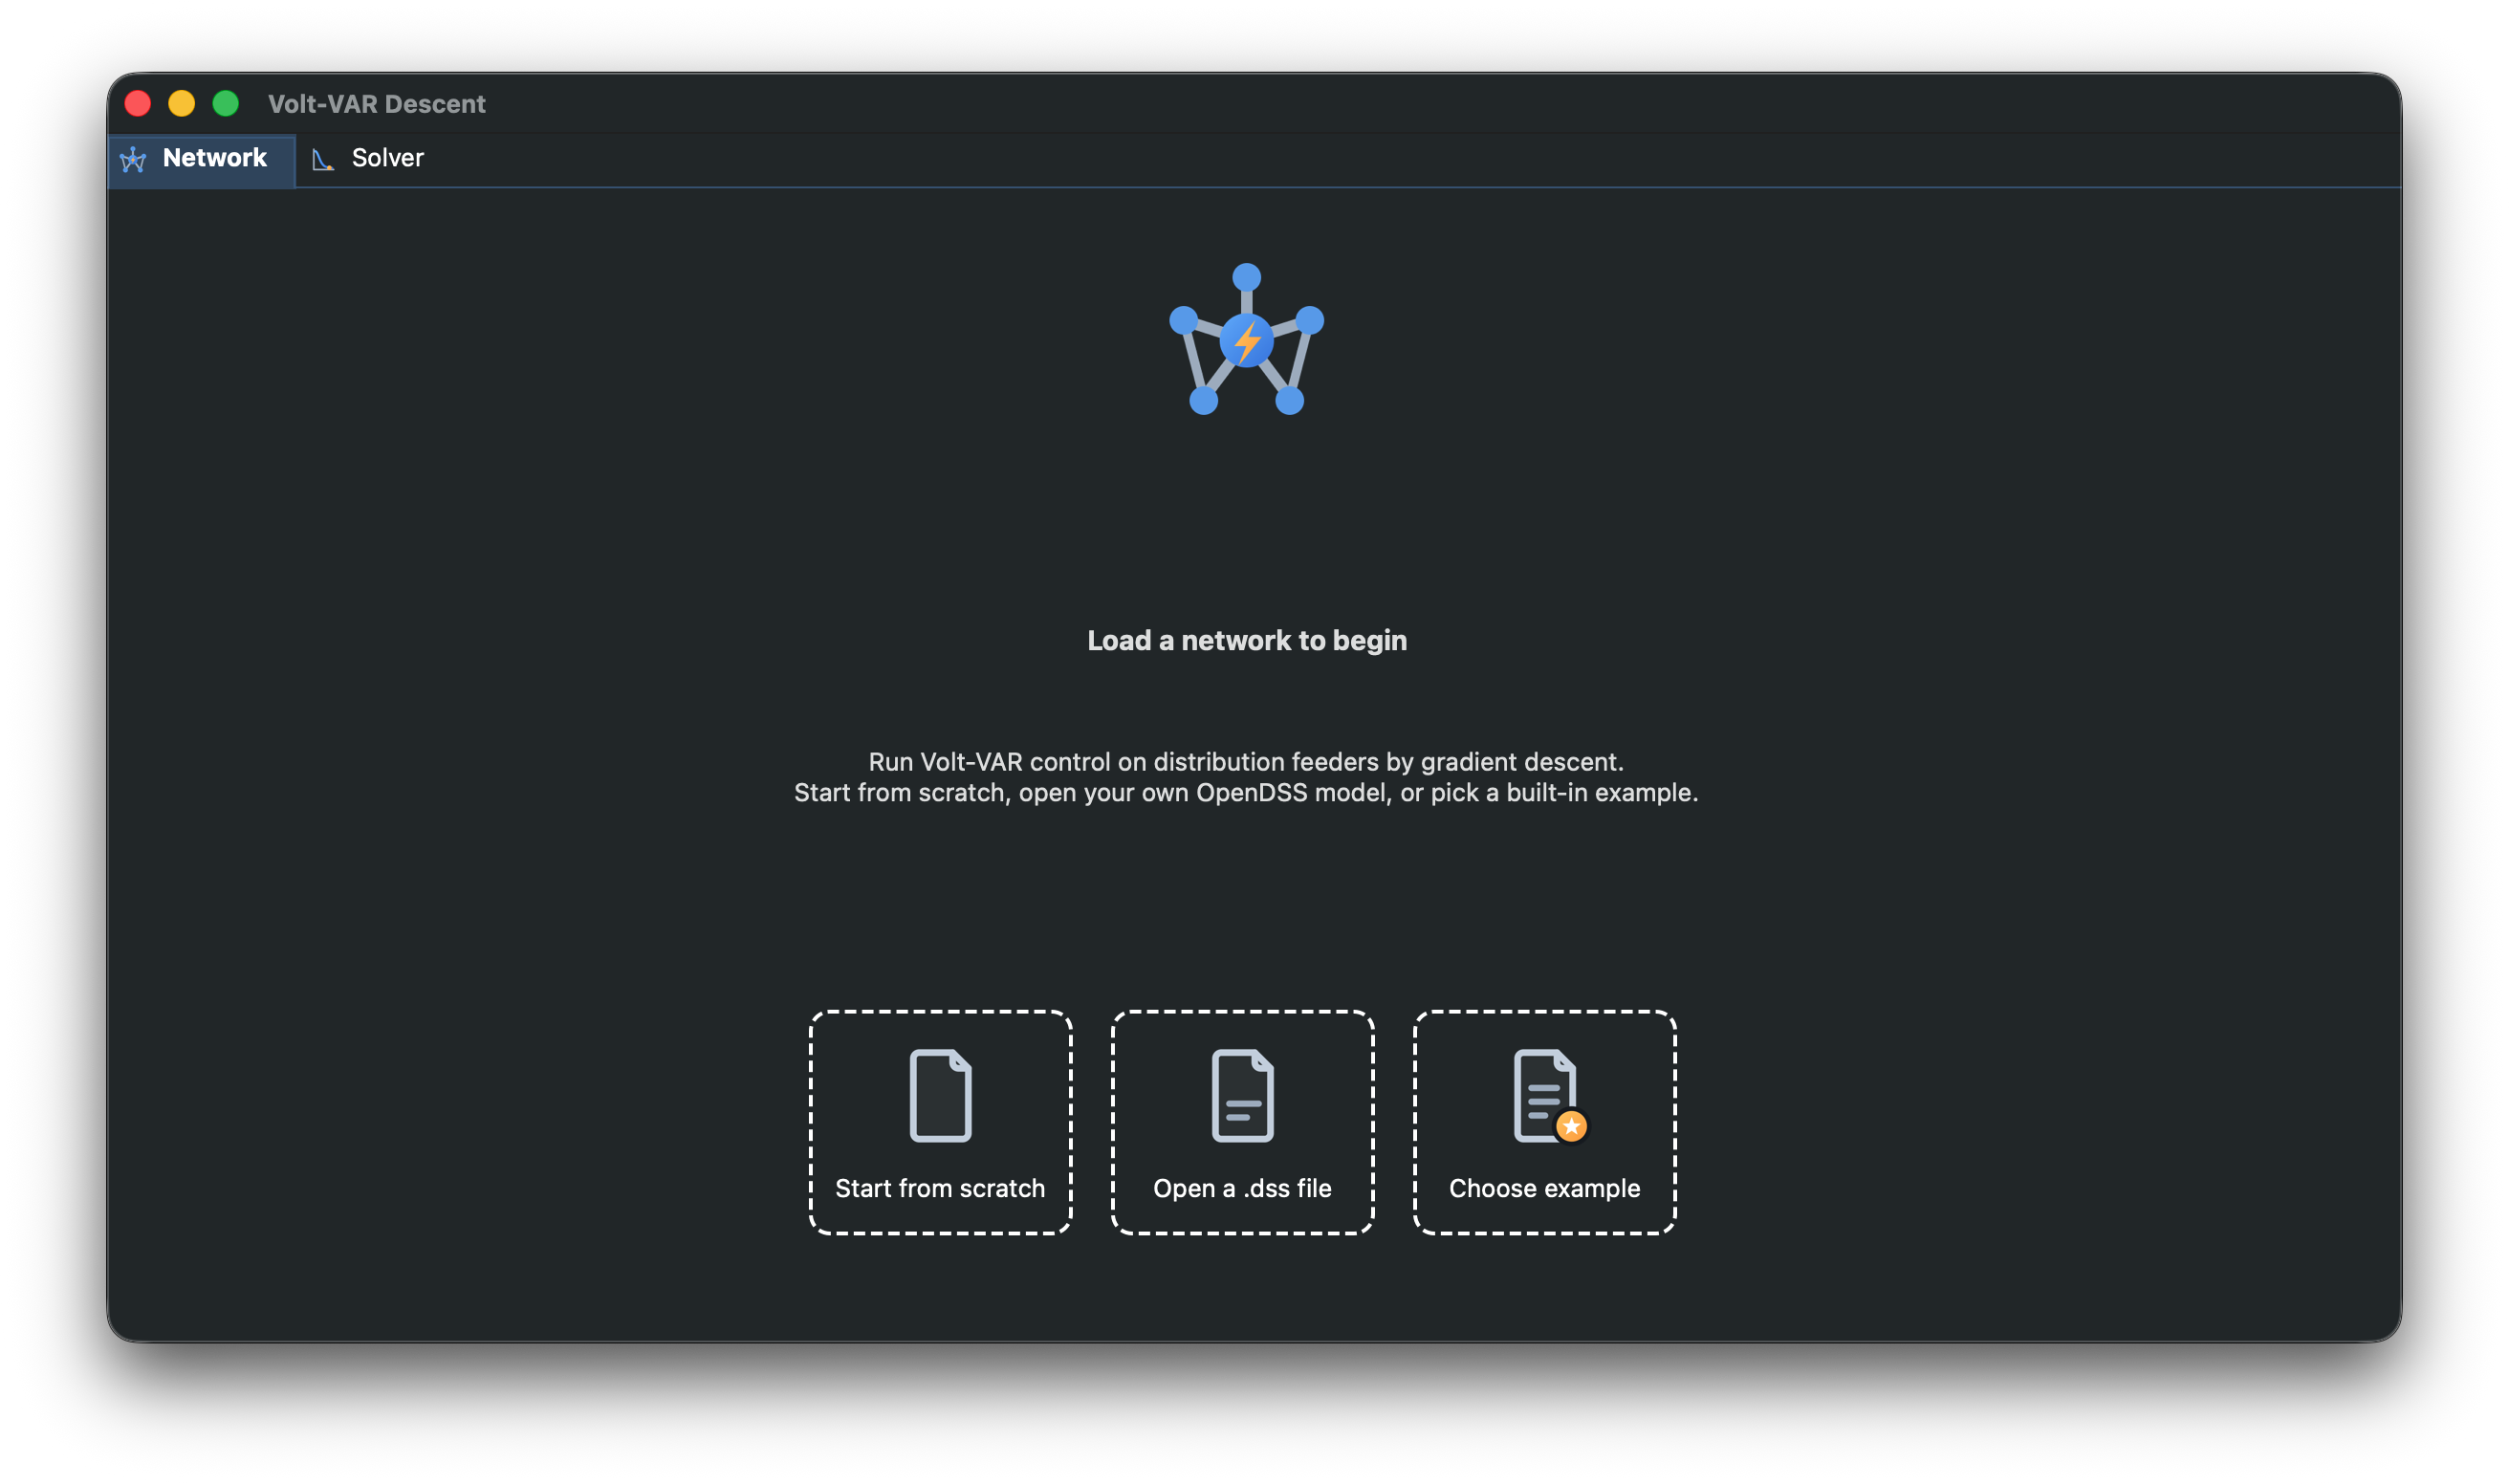
\includegraphics[width=1\textwidth]{assets/network_tab.png}
\caption{Početni prikaz}
\label{fig:network-tab}
\end{figure}

Jedna od prednosti aplikacije je mogućnost brzog pokretanja ugrađenih testnih primjera. Na taj način korisnik ne mora odmah pisati vlastiti OpenDSS model, nego može provjeriti rad aplikacije nad već pripremljenim mrežama sa jednim, dva ili tri PV sistema.

\begin{figure}[H]
\centering
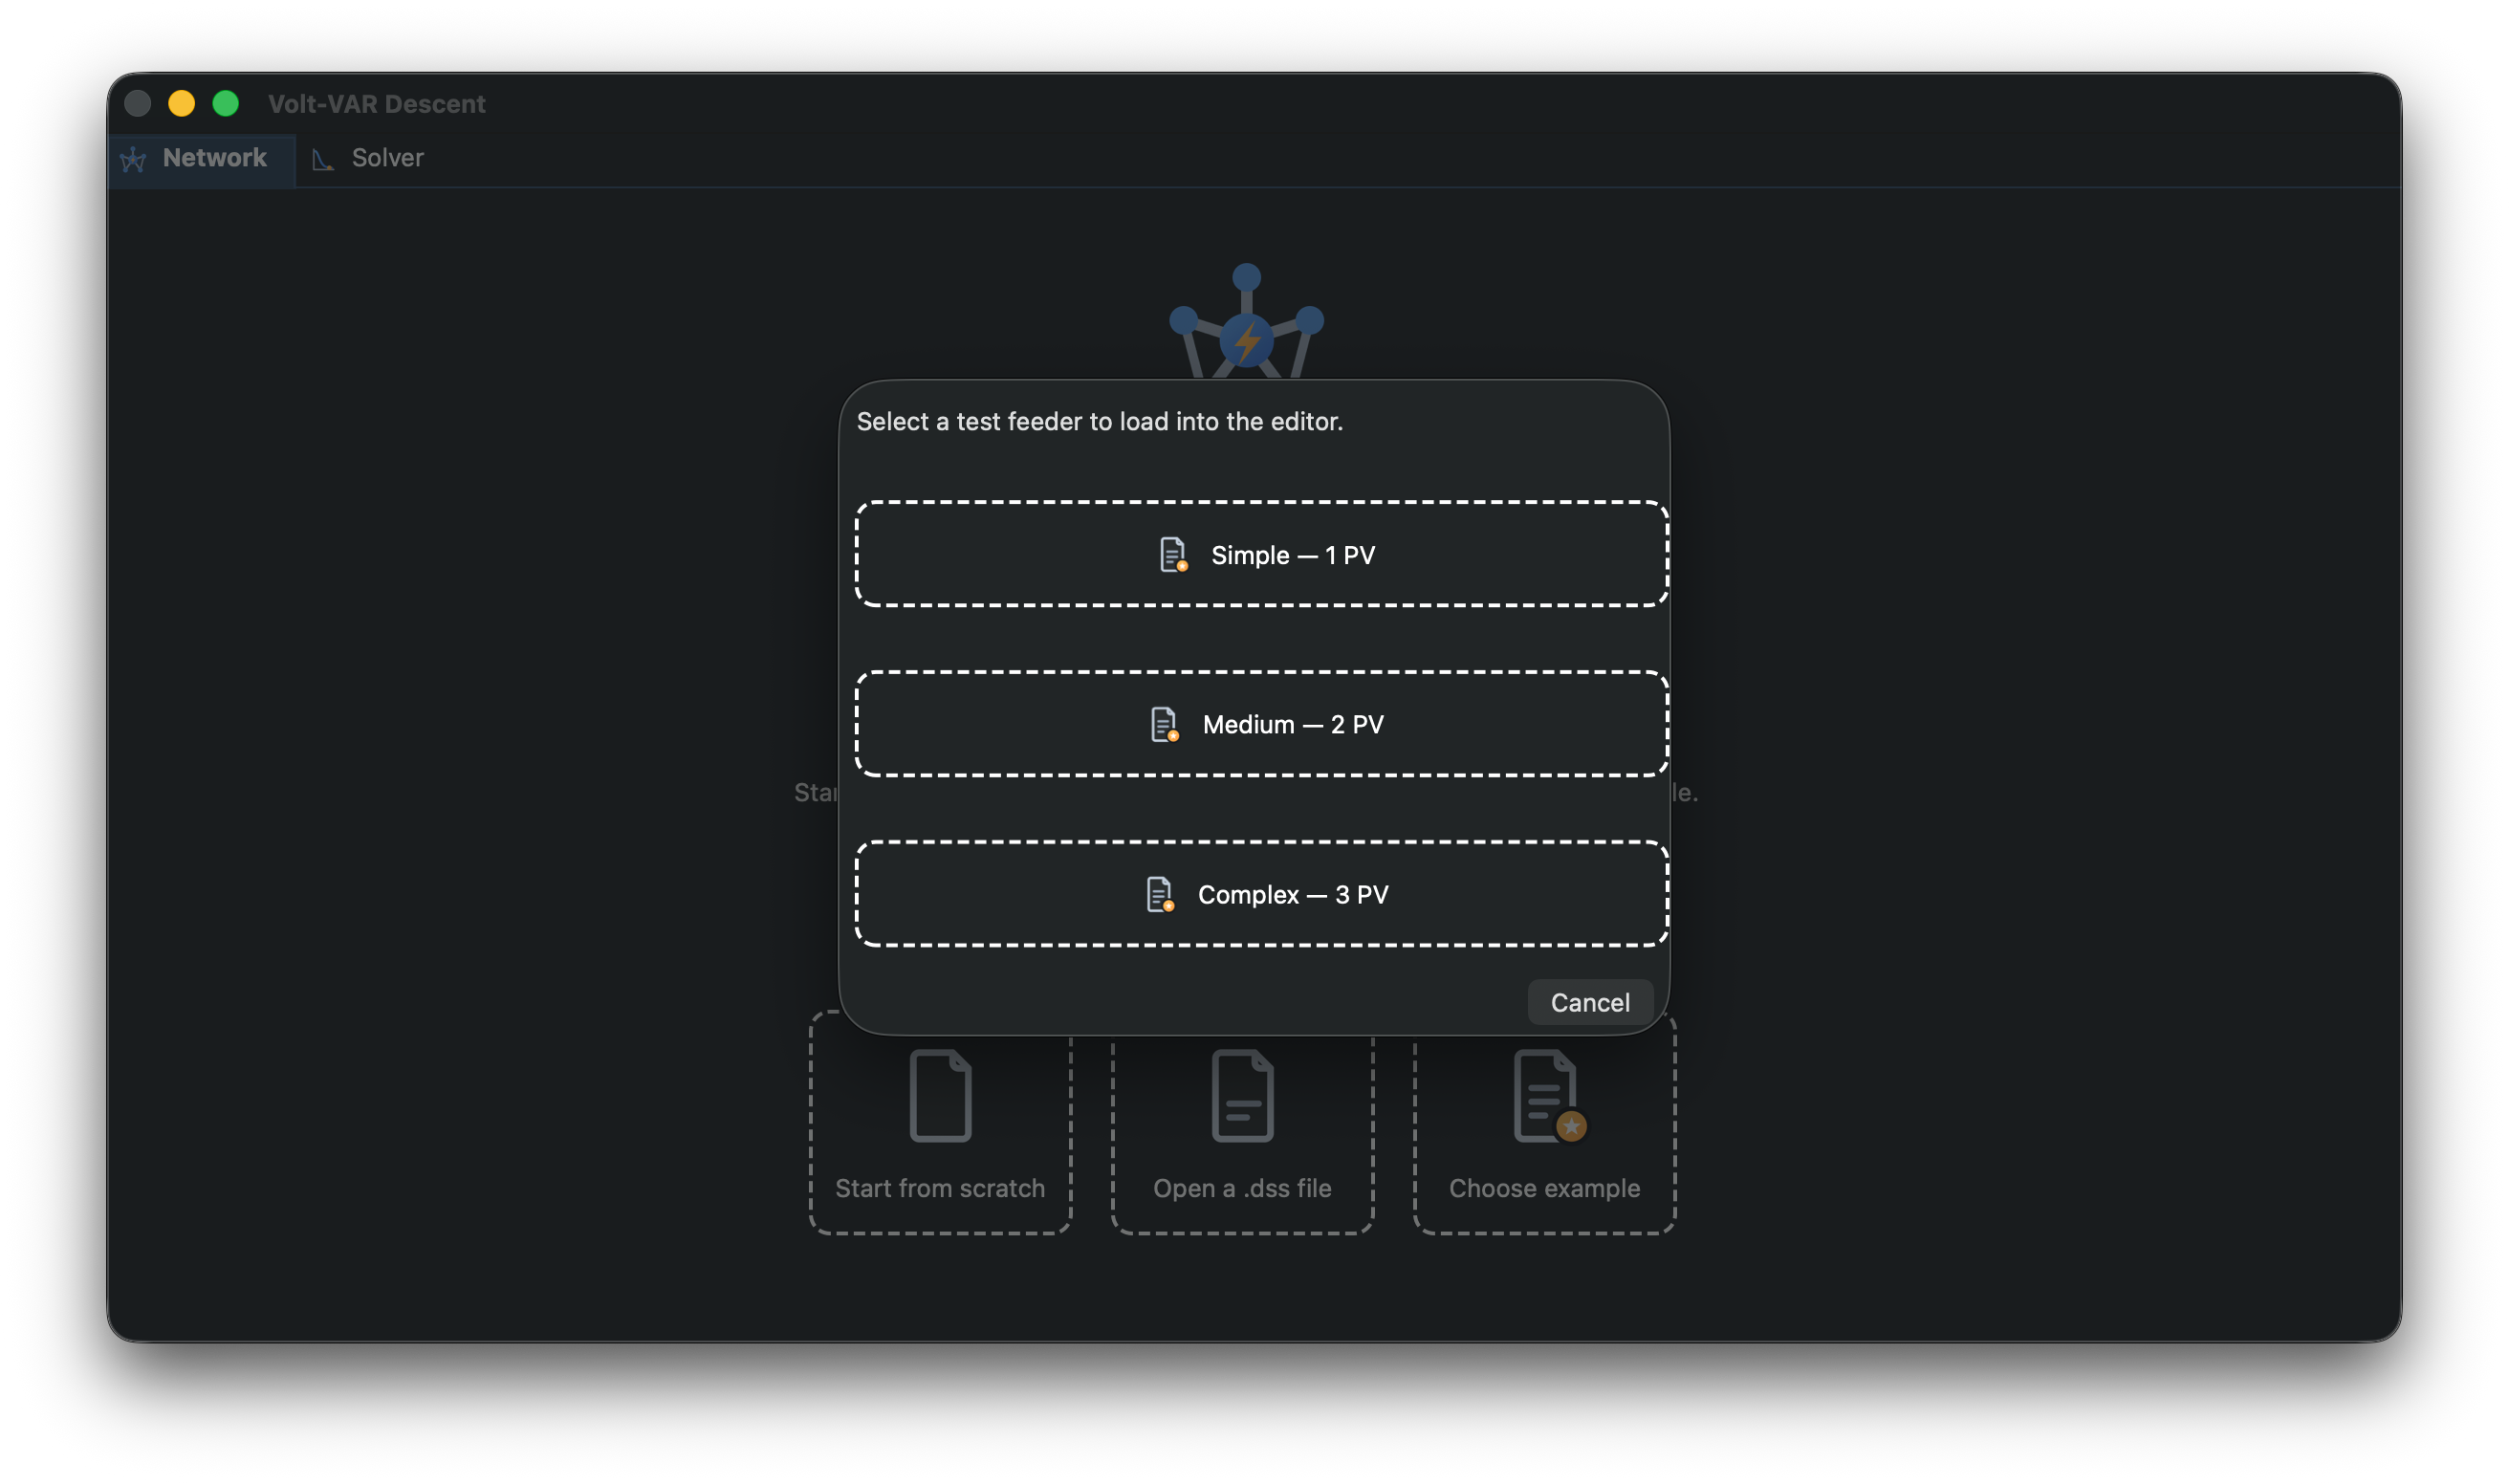
\includegraphics[width=1\textwidth]{assets/network_tab_example.png}
\caption{Odabir ugrađenog primjera}
\label{fig:network-tab-example}
\end{figure}

Nakon učitavanja primjera ili otvaranja datoteke, OpenDSS skripta se prikazuje u tekstualnom editoru. Korisnik može pregledati model, izmijeniti parametre mreže i zatim pokrenuti validaciju. Klikom na dugme za validaciju, skripta se prosljeđuje OpenDSS-u, gdje se provjerava da li je model moguće ispravno učitati i riješiti.

Ako je validacija uspješna, aplikacija prikazuje kratak sažetak mreže. U njemu se nalaze osnovni podaci o modelu, kao što su broj sabirnica, čvorova, vodova, opterećenja, transformatora, kondenzatora, generatora i PV sistema. Ako korisnik nakon validacije promijeni sadržaj skripte, validacija se poništava i \textit{Solver} tab se zaključava dok se mreža ponovo ne validira.

\begin{figure}[H]
\centering
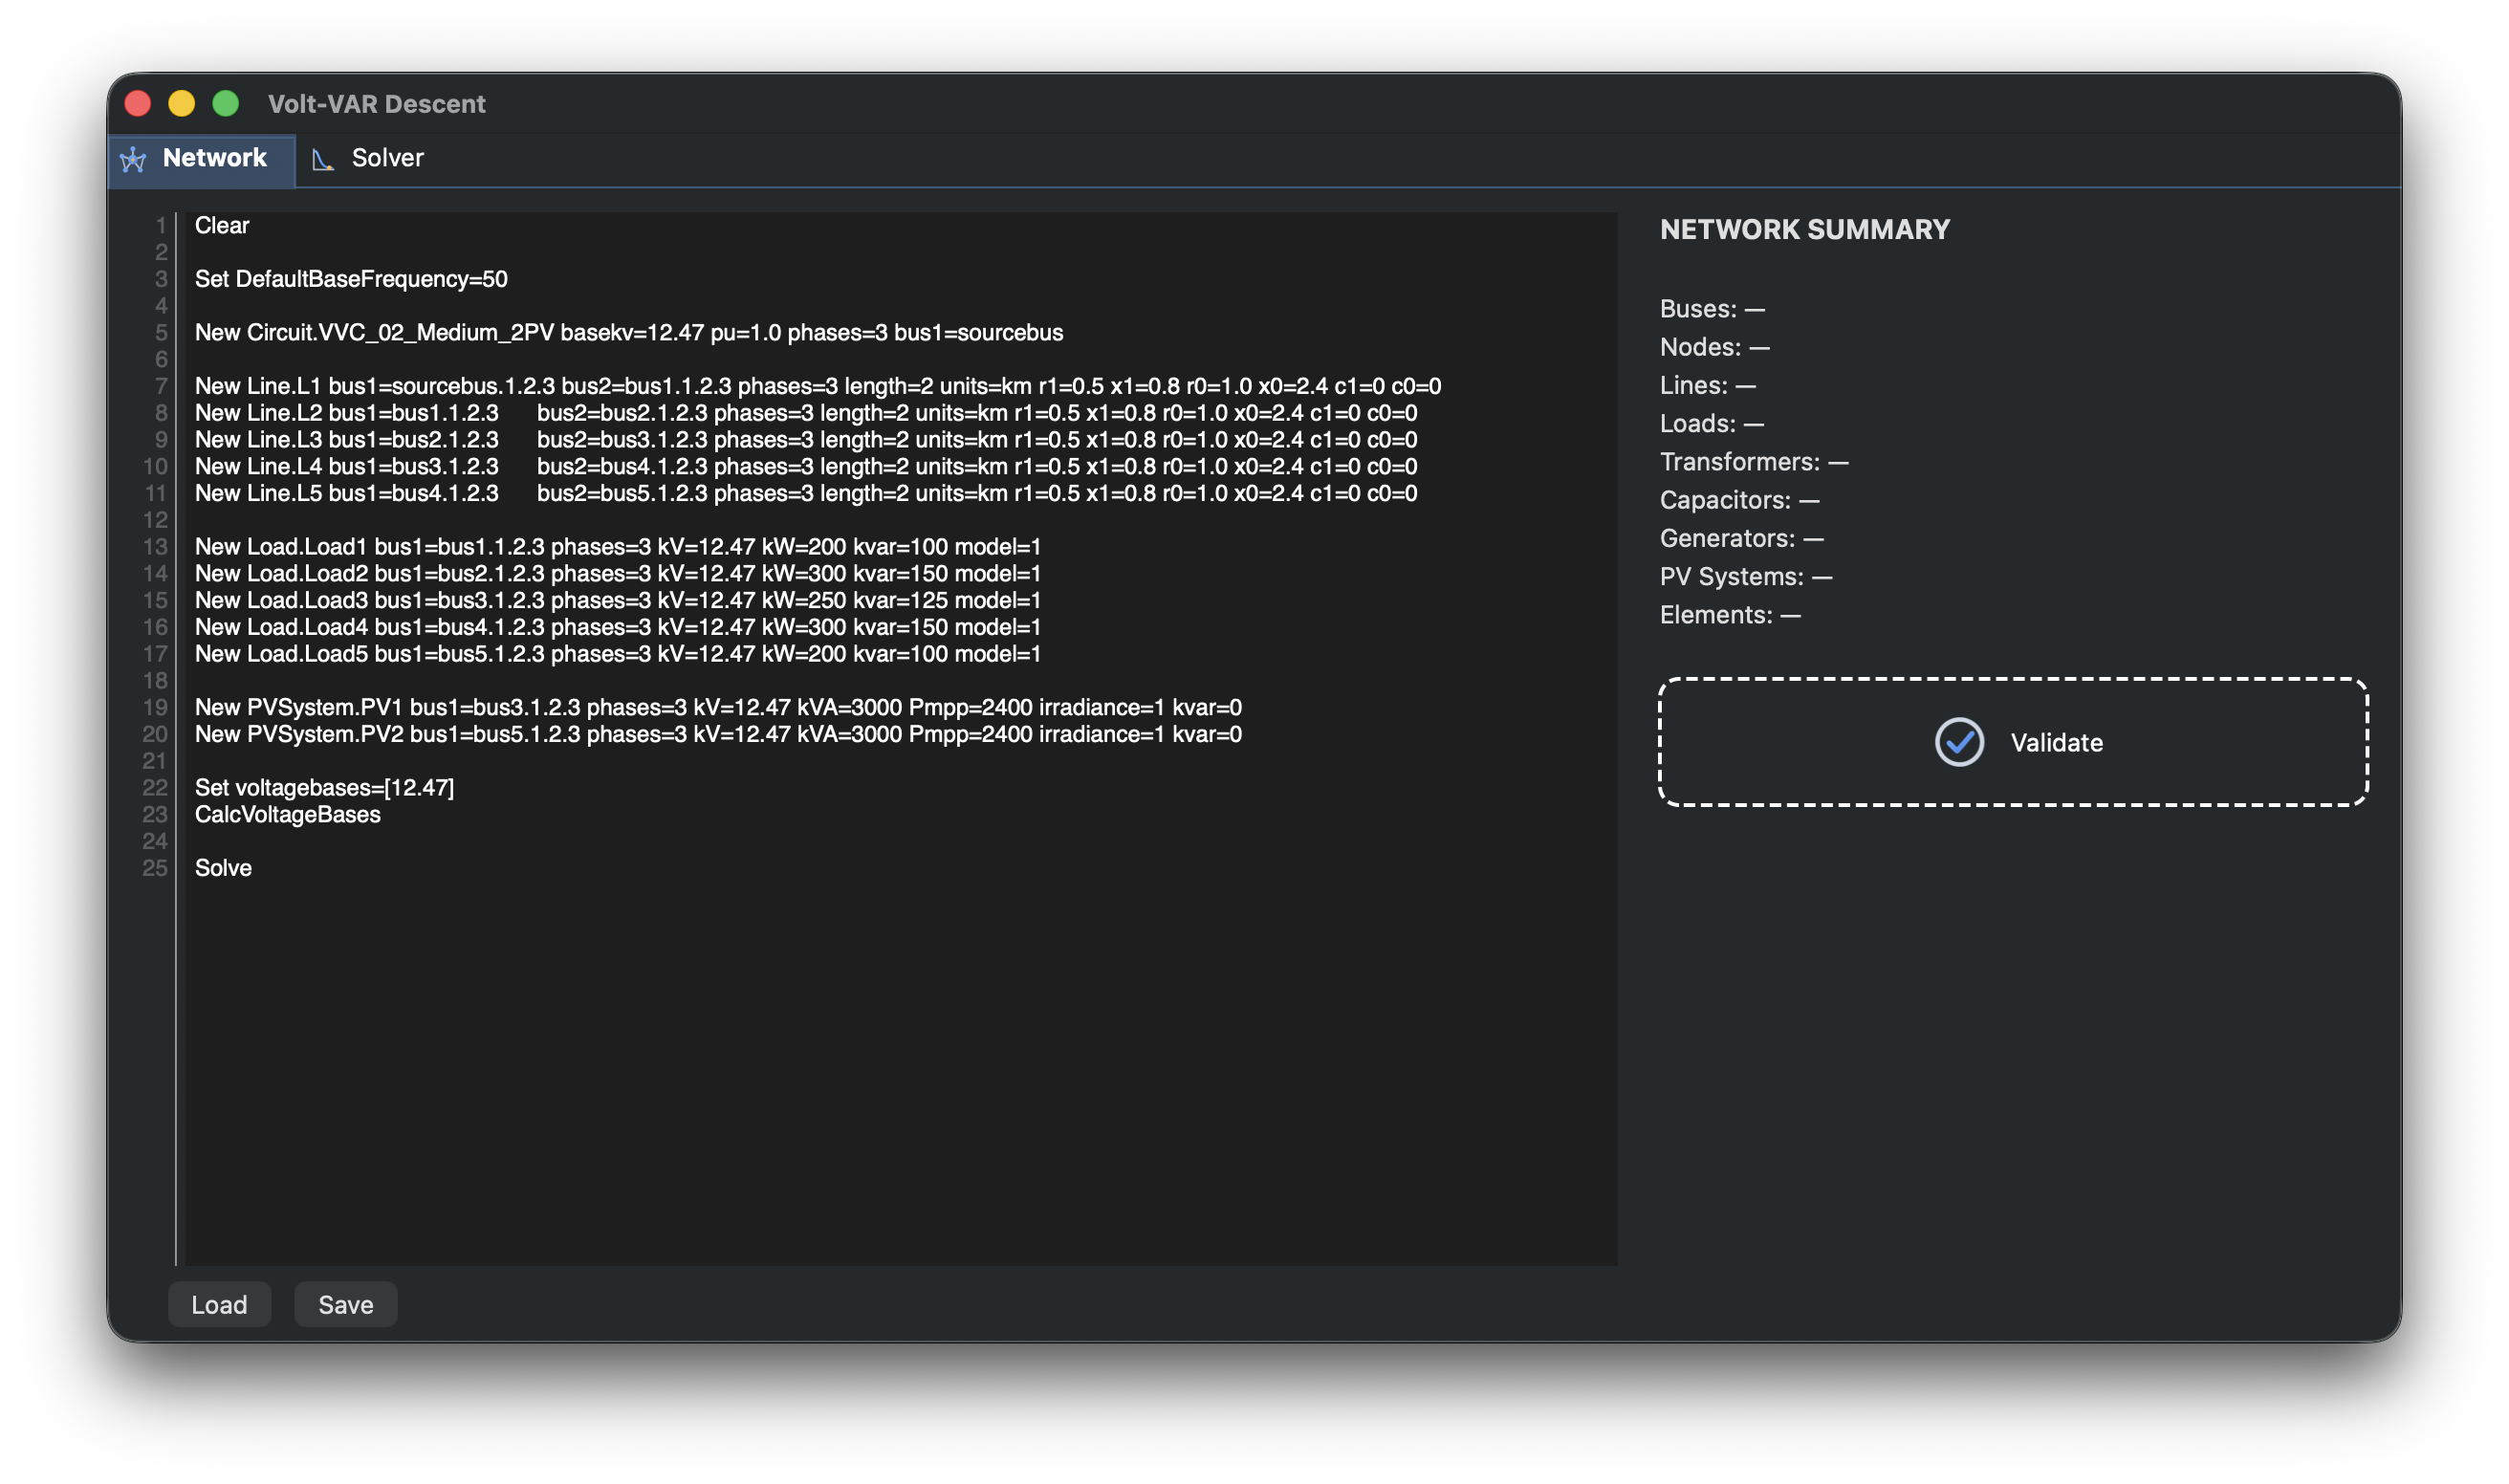
\includegraphics[width=1\textwidth]{assets/network_tab_editor.png}
\caption{Editor OpenDSS skripte i sažetak mreže}
\label{fig:network-tab-editor}
\end{figure}

\section{Solver tab}

Nakon uspješne validacije mreže, korisniku postaje dostupan sadržaj \textit{Solver} taba. U ovom dijelu aplikacije podešavaju se parametri optimizacije i pokreće algoritam gradijentnog spusta.

Korisnik može podesiti maksimalan broj iteracija, brzinu učenja, maksimalni korak promjene reaktivne snage, korak za numeričku procjenu gradijenta, granicu reaktivne snage invertera i toleranciju konvergencije. Nakon podešavanja parametara, solver se pokreće klikom na dugme \textit{Pokreni solver}.

Rezultati se prvo prikazuju u tekstualnom obliku. Izvještaj sadrži početne napone, vrijednosti funkcije troška kroz iteracije, promjene reaktivne snage PV sistema i konačno stanje mreže nakon optimizacije.

\begin{figure}[H]
\centering
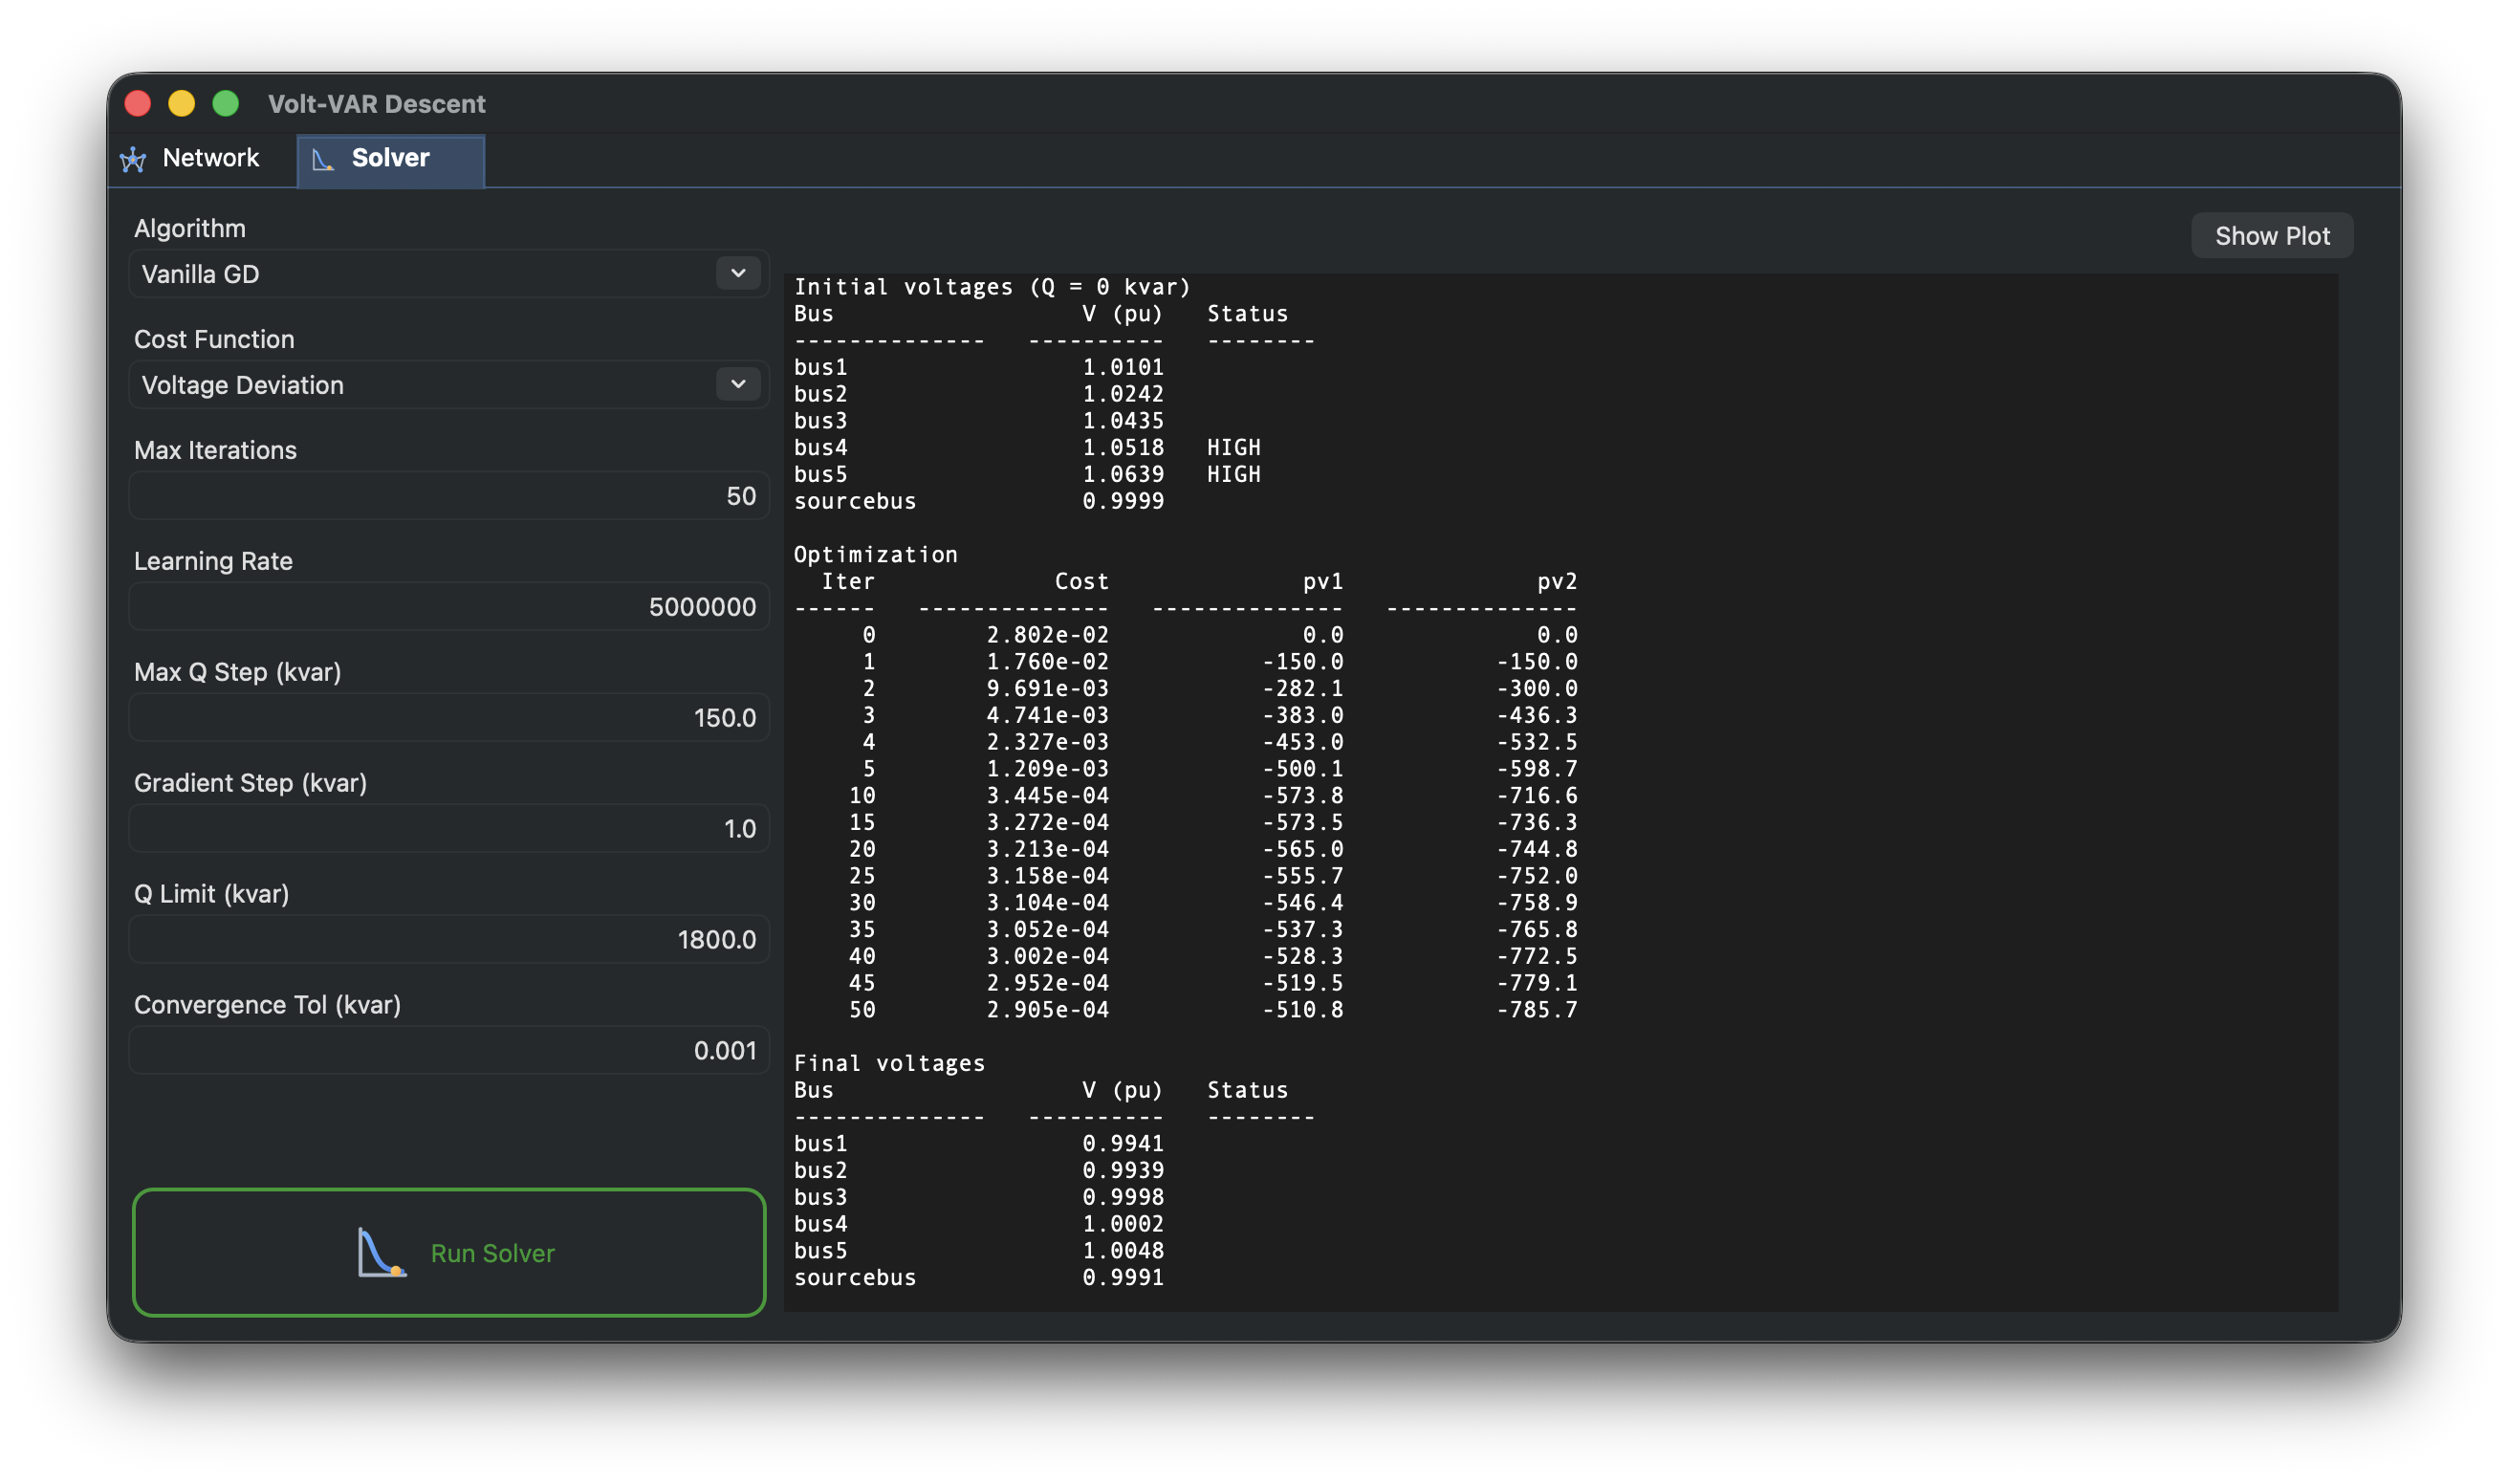
\includegraphics[width=1\textwidth]{assets/solver_text.png}
\caption{Tekstualni prikaz rezultata}
\label{fig:solver-text}
\end{figure}

Pored tekstualnog izvještaja, aplikacija omogućava i grafički prikaz promjene reaktivne snage. Na dijagramu je za svaki PV sistem prikazana posebna kriva, i na osnovu ovog prikaza može se vidjeti da li se vrijednosti $Q$ stabiliziraju i da li algoritam konvergira prema konačnom rješenju.

\begin{figure}[H]
\centering
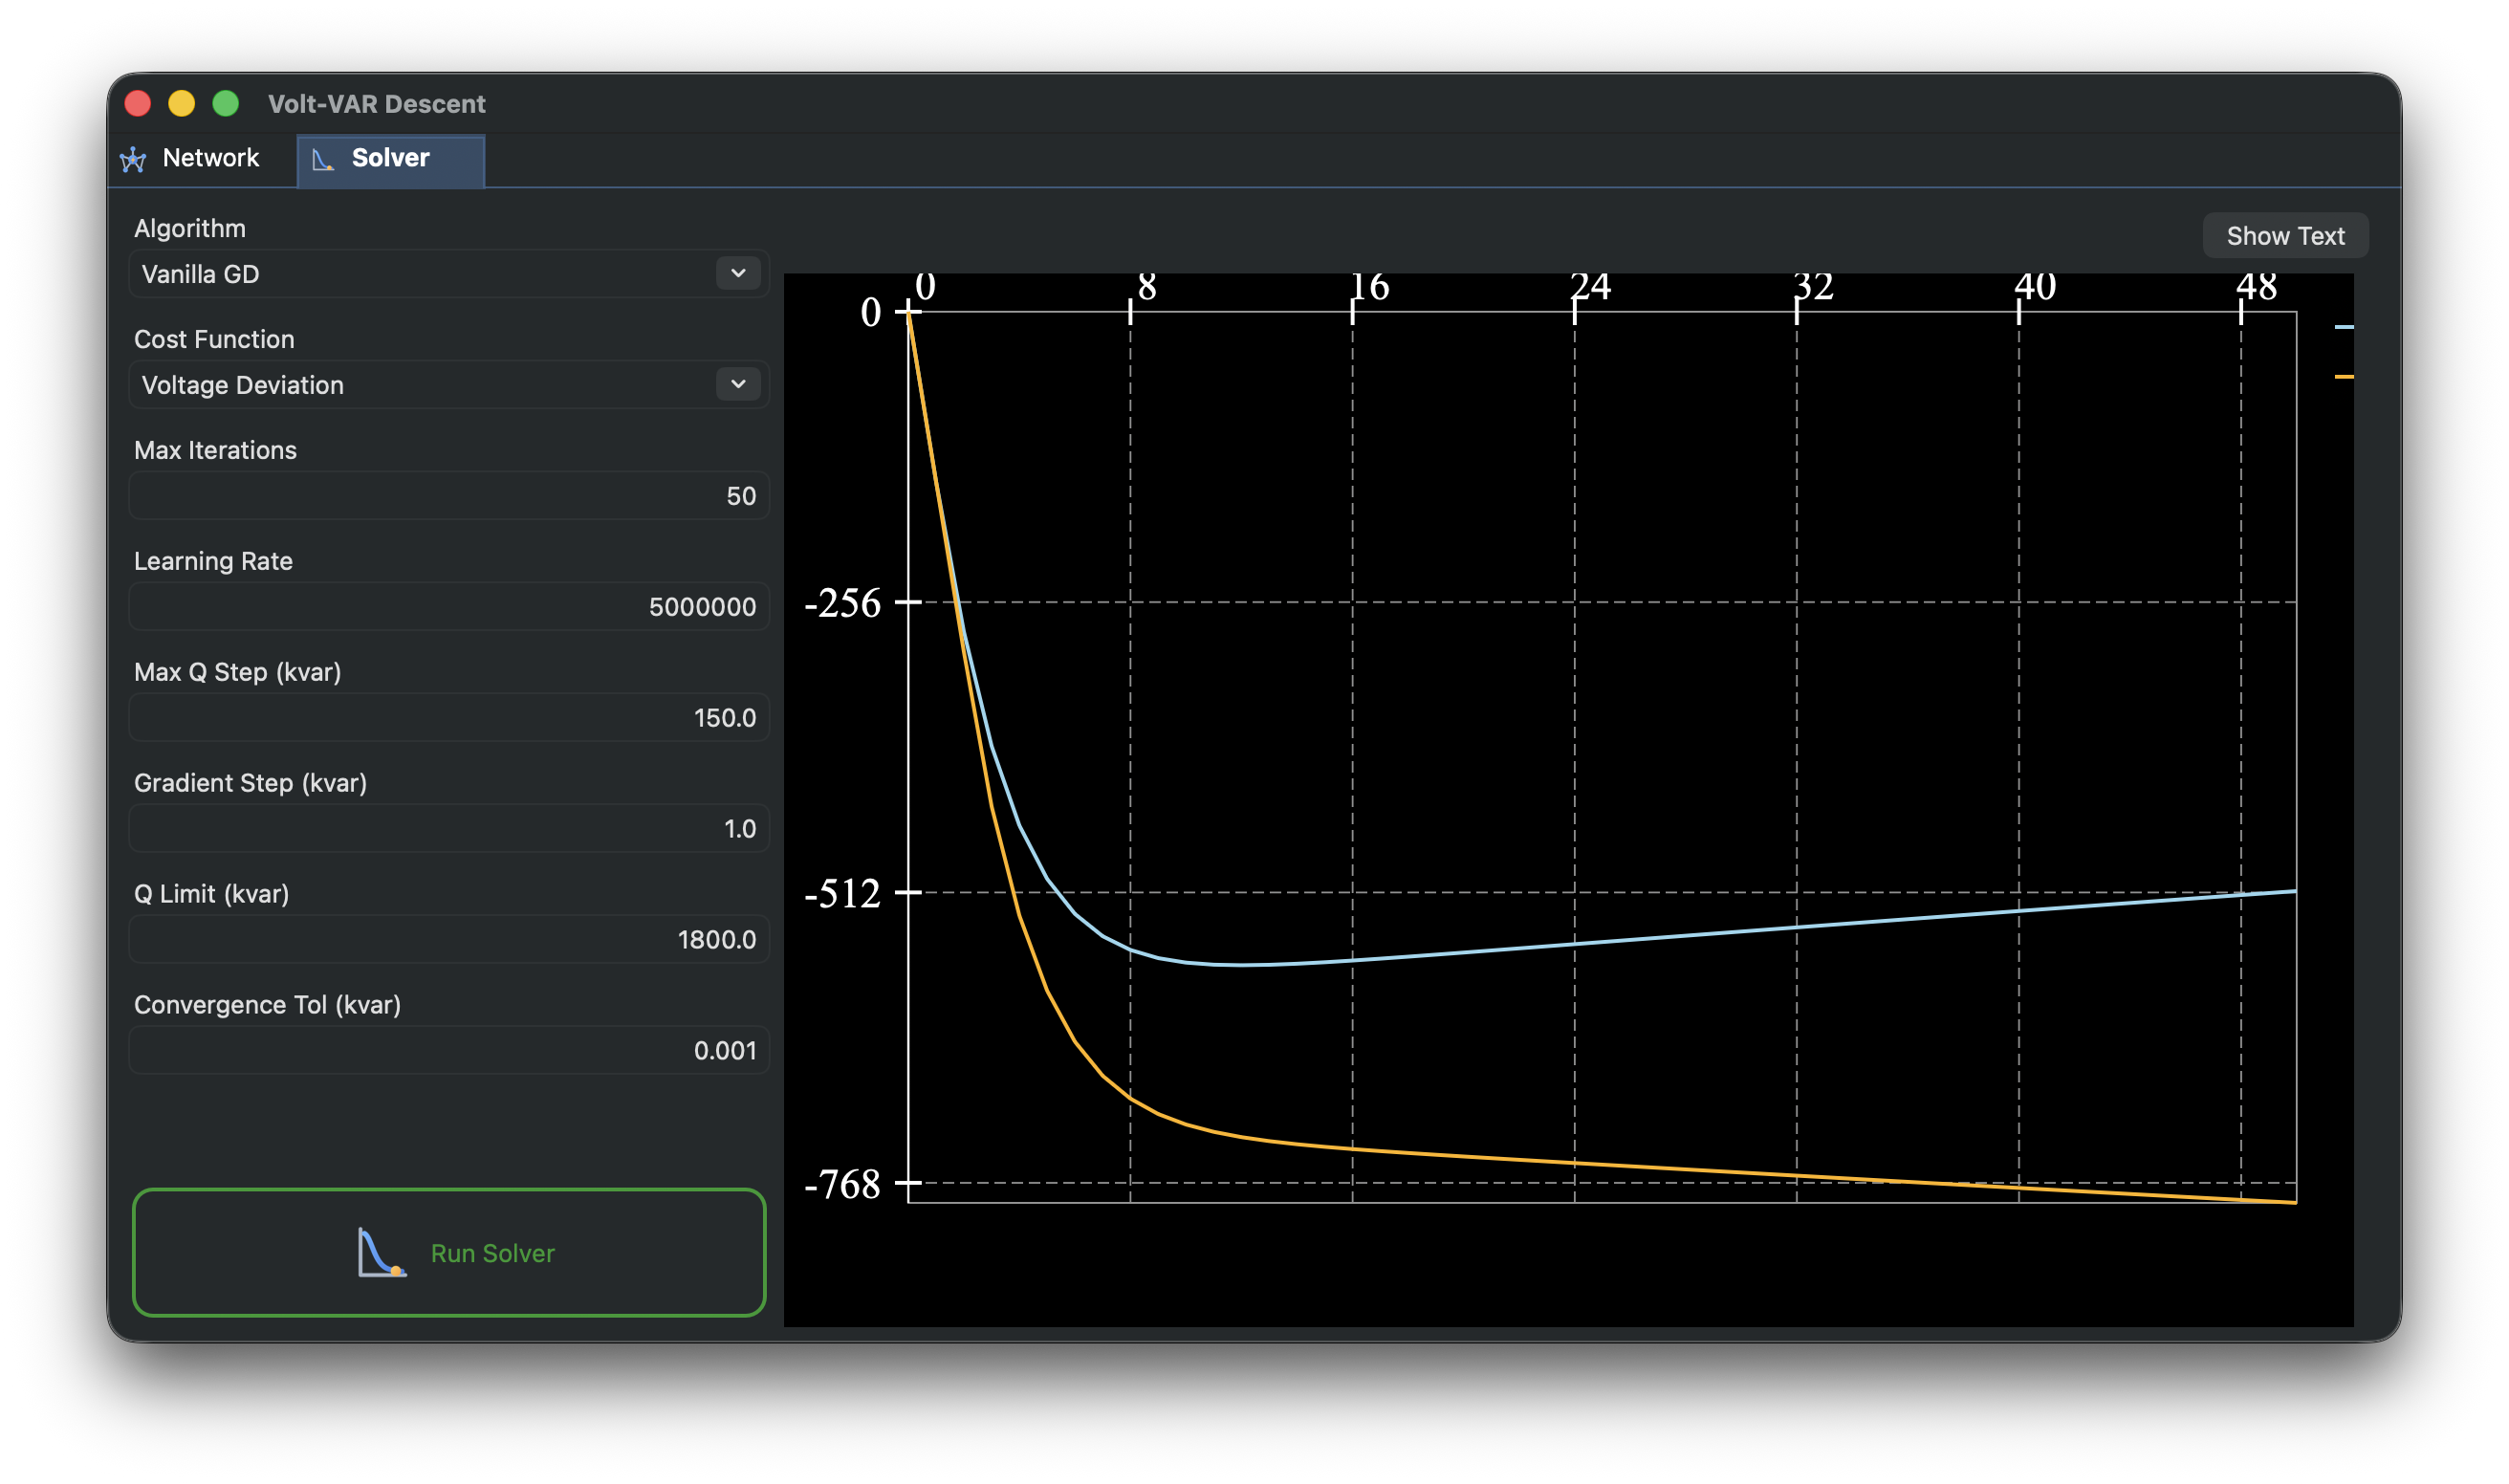
\includegraphics[width=1\textwidth]{assets/solver_plot.png}
\caption{Grafički prikaz promjene reaktivne snage}
\label{fig:solver-plot}
\end{figure}

\chapter{Zaključak}

U ovom radu implementirana je aplikacija \textbf{Volt-VAR Descent}, namijenjena za određivanje Volt-VAR kontrole u distributivnim mrežama sa PV sistemima. Aplikacija je implementirana kao C++ desktop aplikacija i omogućava korisniku da učita OpenDSS model mreže, validira ga, podesi parametre optimizacije i pokrene algoritam gradijentnog spusta.

Za rješavanje toka snage korišten je OpenDSS preko biblioteke \texttt{dss\_capi}, dok je optimizacijski dio implementiran unutar aplikacije. Gradijent funkcije troška računa se numerički tako što se za svaki PV sistem posmatra uticaj male promjene reaktivne snage na mrežu. Na osnovu izračunatog gradijenta mijenjaju se vrijednosti reaktivne snage $Q$.

Implementirano rješenje pokazuje kako se jednostavan algoritam gradijentnog spusta može koristiti za interaktivno određivanje Volt-VAR kontrole. Iako korišteni pristup nije najbrži za veće mreže, jer zahtijeva više računanja tokova snage u svakoj iteraciji, prednost mu je jednostavna implementacija i mogućnost rada nad proizvoljnim OpenDSS modelom bez dodatnog izvođenja analitičkih osjetljivosti.

Aplikacija ispunjava osnovne zahtjeve rada: koristi C++, natID GUI, natID guste matrice za numeričke podatke, CMake konfiguraciju i podršku za višeplatformsko pokretanje. Kao moguća dalja unapređenja ostaju implementacija dodatnih funkcija troška, dodatne verzije algoritma gradijentnog spusta i proširenje testiranja na složenije distributivne mreže.


\begin{thebibliography}{9}


\bibitem{sensitivity_vvc}
R. A. Jabr and I. Džafić, 
\textit{Sensitivity-based discrete coordinate-descent for Volt/VAr control in distribution networks}, 
IEEE Transactions on Power Systems, 2016.

\bibitem{realtime_gfm_vvc}
R. Wagle, P. Sharma, C. Sharma, M. Amin and F. Gonzalez-Longatt, 
\textit{Real-time Volt-Var control of grid forming converters in DER-enriched distribution network}, 
Frontiers in Energy Research, 2023.

\bibitem{opendss}
EPRI, \textit{OpenDSS -- Open Distribution System Simulator}, 
\url{https://www.epri.com/OpenDSS}.

\bibitem{dsscapi}
DSS-Extensions, \textit{dss\_capi -- OpenDSS C API}, 
\url{https://github.com/dss-extensions/dss_capi}.


\end{thebibliography}

\end{document}
